\section{Implementation}
\label{section:bcoollengbench}
This section presents the implementation of \bcool into the GEMOC studio\footnote{\url{http://www.gemoc.org}}; which integrates technologies based on Eclipse Modeling Framework (EMF)~\footnote{\url{http://eclipse.org/modeling/emf/}} adequate for the specification of executable domain specific modeling languages. The studio includes a \emph{language workbench} to design and implement tool-supported DSMLs and a \emph{modeling workbench} where the DSMLs are automatically deployed to allow designers to edit, execute and animate their models~\cite{ttc15bib}.

\begin{figure}
	\begin{center}
		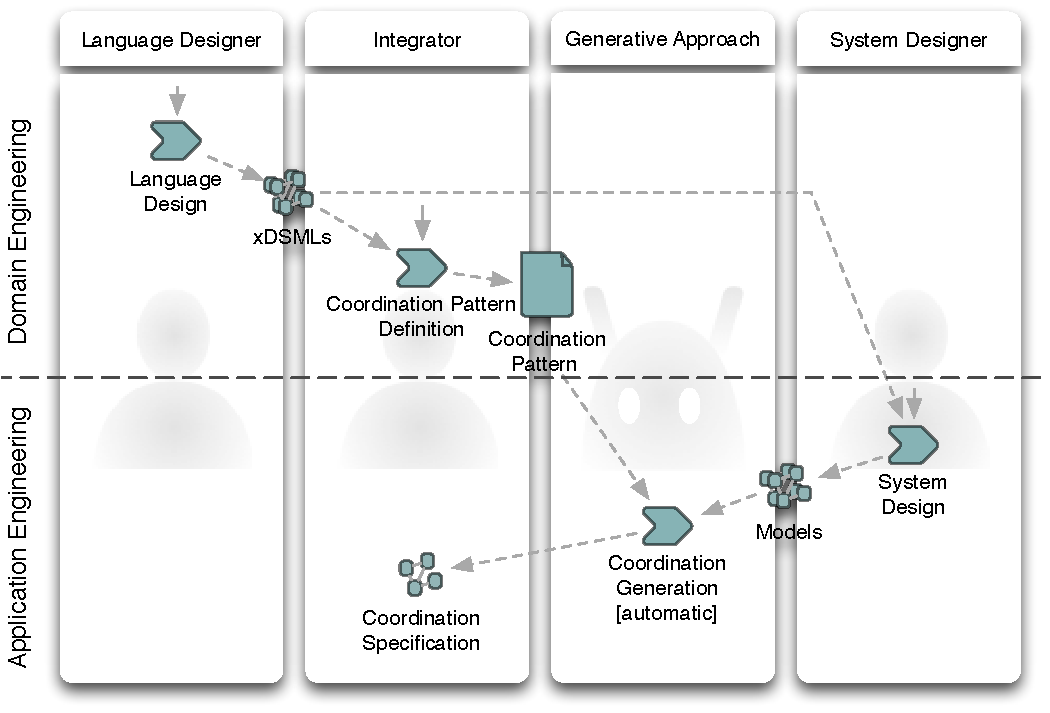
\includegraphics[width=.6\textwidth]{bcool/figs/process}
		\caption{The proposed workflow for the heterogeneous development of complex applications}
		\label{fig:proposedworkflow}
	\end{center}
\end{figure}

\bcool takes advantages of this collaborative environment by adding coordination facilities. Figure~\ref{fig:proposedworkflow} illustrates the proposed workflow in which a language integrator uses the language workbench to develop \bcool operators to specify coordination patterns between languages. Then, a system designer can use these operators in the modeling workbench to coordinate models. In this section, we illustrate the use of the language workbench by developing the running example operator (see Listing~\ref{lst:bcoolrunningexample}). Then, in the modeling workbench, we use this operator to execute and verify the models of the coffee machine. 

\begin{figure}[]
	\begin{center}
		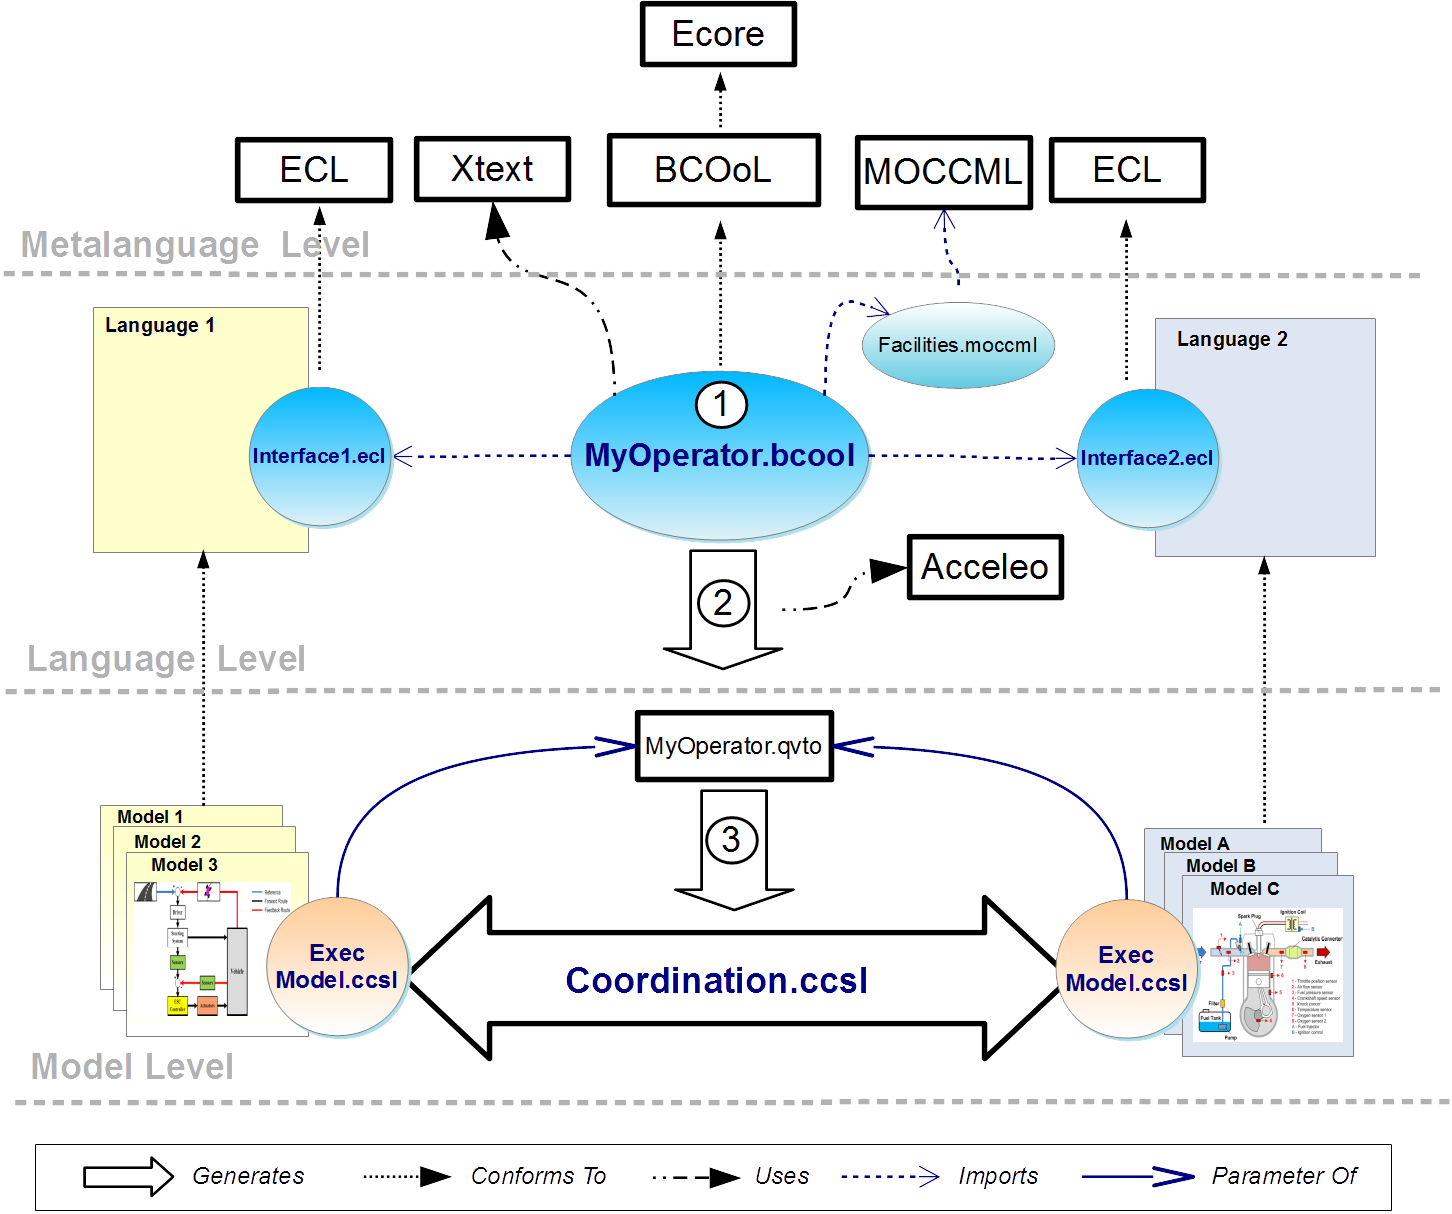
\includegraphics[width=1\textwidth]{bcool/figs/bcooltechnos}
		\caption{Overview of the implementation of \bcool and its integration into the Gemoc Studio}
		\label{fig:bcooltechnos}
	\end{center}
\end{figure}

\bcool is developed as a set of plugins based on the EMF (at top of Figure~\ref{fig:bcooltechnos}). The \bcool abstract syntax has been developed using Ecore (\ie the metalanguage associated with EMF) and the textual concrete syntax has been developed in Xtext~\footnote{http://eclipse.org/Xtext/}, thus providing advanced editing facilities. For the running example operator, we use the TFSM and Activity languages that are integrated into the studio. Then, we use \bcool to specify the Listing~\ref{lst:bcoolrunningexample} (Figure~\ref{fig:bcooltechnos}: step 1). In the \bcool specification, we can import the language behavioral interfaces of each language deployed in the language workbench. In addition, the language workbench provides \moccml thus helping the integrator to specify relations and expression.      

%When languages are deployed into the language workbench, an integrator can define a new \bcool specification and then import the language behavioral interfaces that are automatically deployed (Figure~\ref{fig:bcooltechnos}: step 1). Also, the language workbench provides \moccml thus helping the integrator to specify relations and expression. For the running example, we use the TFSM and Activity languages that are integrated into the studio. 

In the modeling workbench, a system designer can use \bcool operators to automate the coordination of models and to execute the coordinated system. To do so, a system designer has to specify a \bflow specification (Figure~\ref{fig:bcooltechnos}: step 2), and then, uses it to launch the \emph{Gemoc Coordinated Execution Engine} (Figure~\ref{fig:bcooltechnos}: step 3). In the following, we elaborate on these two tasks.  

We provide a simple language named \bflow (standing for \bcool \emph{FL}o\emph{W}) that enables a system designer to specify how operators of a \bcool specification are applied on a set of models (Figure~\ref{fig:bcooltechnos}: step 2). To introduce \bflow, Listing~\ref{lst:bflowcoffeemachine} shows the specification for the models of the coffee machine. It begins by importing the \bcool specification that contains the operators (Listing~\ref{lst:bflowcoffeemachine}: line 2). Then, it specifies the models that will be coordinated. For the running example, this corresponds with the TFSM named \emph{CoffeeCoin.tfsm} and the Activity named \emph{CoffeAlgorithm.ad} (Listing~\ref{lst:bflowcoffeemachine}: line 3 and 4). Then, the specification contains a \emph{Flow} that defines which operators are used and on which models are applied. A Flow defines a sequential order of application of operators. In other words, the first line is the first operator that will be applied and soon on. For instance, in Listing~\ref{lst:bflowcoffeemachine}, line 6 specifies that the operator named \emph{SyncFMEventsAndActions} must be applied between the models CoffeeCoin and CoffeeAlgorithm. This corresponds with the first and the only operator to be applied to coordinate the models of the coffee machine. However, a \bflow specification may use several operators depending on the number of models in the system, this is further discussed in Chapter~\ref{ch:examples}.  

\begin{lstlisting}[language=bflow,
caption={\bflow specification for the models of the coffee machine},
label={lst:bflowcoffeemachine}, 
basicstyle=\scriptsize\ttfamily, backgroundcolor=\color{LGrey}, numbers=left, xleftmargin=2pt]
BCOoLFlow CoffeeMachine
ImportBCOoL  "TFSMAndActivity.bcool" ;
Model CoffeCoin "coffeecoin.tfsm"
Model CoffeeAlgorithm "coffeeAlgorithm.ad"
Flow 
	applies SyncFSMEventsAndActions between (CoffeeAlgorithm, CoffeCoin);
end Flow;
\end{lstlisting}


The Gemoc Coordinated Execution Engine uses the \bflow specification to generate a model of coordination that is used to execute the coordinated system. The generation is implemented by using a high-order transformation in Acceleo~\footnote{\url{http://www.eclipse.org/acceleo/}} that translates the \bcool specification into a QVTo~\footnote{\url{https://projects.eclipse.org/projects/modeling.mmt.qvt-oml}} transformation (\emph{Compilator} in Figure~\ref{fig:bcooltechnos}). Then, the Gemoc Coordinated Engine invokes the generated QVTo transformation which takes as parameters the models to be applied and the operators that must be applied. This information is retrieved from the \bflow specification. The QVTo transformation is finally applied between the corresponding models thus generating a model of coordination in \ccsl. 

To execute the coordinated model, the Gemoc Coordinated Execution Engine first initializes the \emph{Gemoc Execution Engine} of each individual model. These engines compute the next valid step for each model. Also, there is a \emph{Coordination Engine} that computes the next valid step for the coordination. To compute the next \emph{global} valid step, the Gemoc Execution Engine gets the next valid step from each individual engine and from the coordination engine. Then, it selects the possible steps that are valid for both the individual models and the coordination. This results in a set of global valid steps. 

To illustrate the use of the Coordinated Execution Engine, we coordinate and execute the models of the coffee machine. First, we configure the launcher that contains information about the \bcool specification, the \bflow specification and the configuration launcher for each model. In Figure~\ref{fig:execenginemenu}, by clicking on \emph{Debug}, the execution is launched. Then, each individual engine is initialized together with the engine for the coordination (Figure~\ref{fig:runningworkbench}: point 2). The \emph{Concurrent Logical Steps Decider} view provides several options to drive the execution of the models. For instance, it provides a list of the next valid execution steps (Figure~\ref{fig:runningworkbench}: point 3). Also, the workbench provides the animation of models (Figure~\ref{fig:runningworkbench}: point 4). 

The modeling workbench provides tools to analyze the resulting \ccsl specification (Figure~\ref{fig:runningworkbench}: point 1). For example, it is possible to obtain by exploration quantitative results on the scheduling state-space of the coordinated system. The exploration of all schedules can be done explicitly in a state space graph. Any cyclic path in this graph (starting from the initial configuration) represents a valid schedule of the models. Figure~\ref{fig:statespace} shows the resulting state-space exploration for the coordinated model of the coffee machine\footnote{The graph in DOT format can be downloaded from the companion website.}. Each state represents a valid step in the execution. In the transitions, the guards contain the events that tick simultaneously when a transition is taken. For example, in red, the figure shows the transitions that contain the events forced to happen simultaneously by the coordination, \eg \emph{selectCoffee:occurs} and \emph{selectCoffee:executeIt}. For the coffee machine, the state exploration results in 39 states, 405 transitions and no dead-locks.    


\begin{figure}[]
	\centering
	\subfigure[Configuration of the launcher of the Gemoc Coordinated Execution Engine]{
		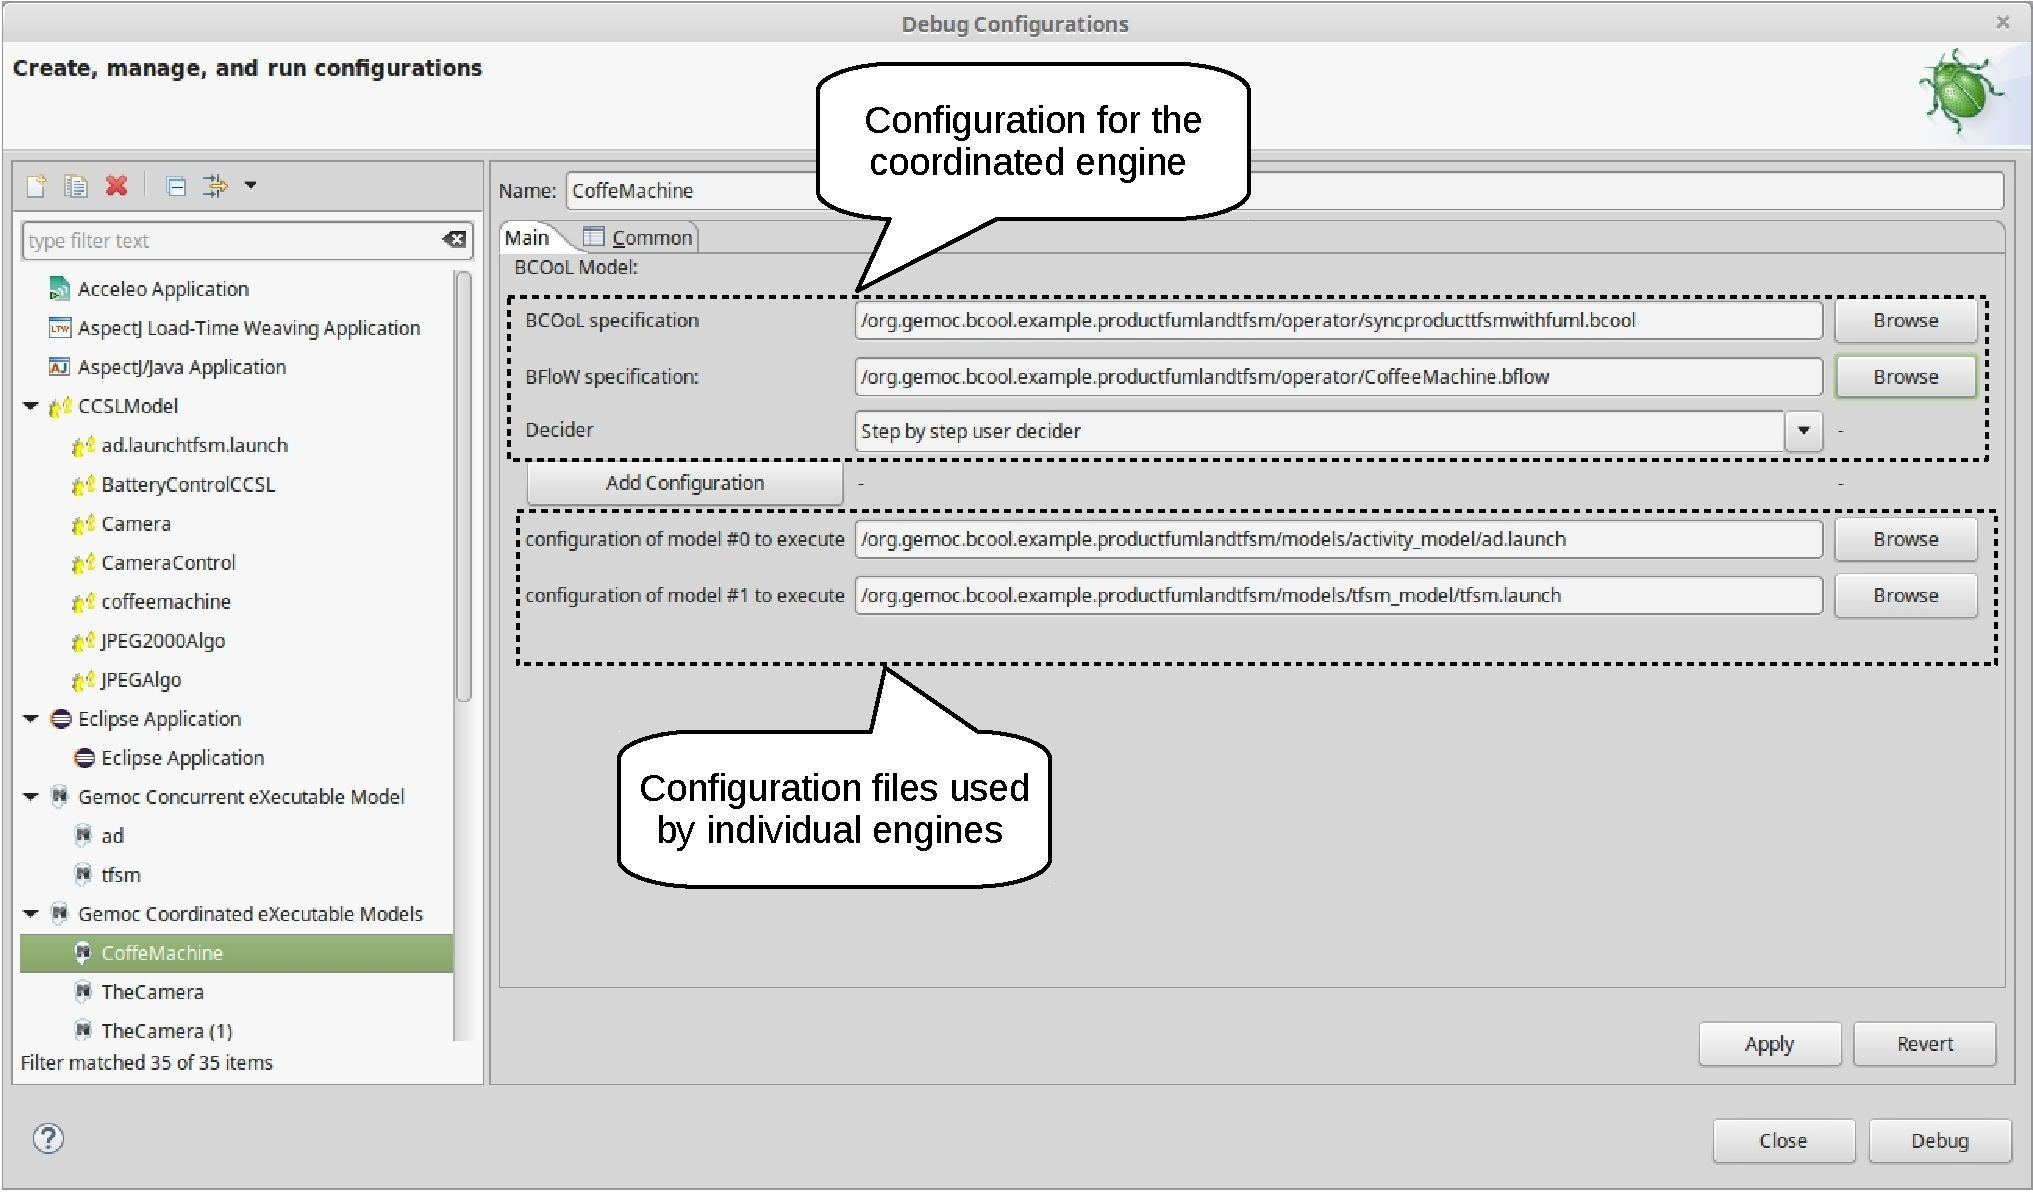
\includegraphics[width=.8\textwidth]{bcool/figs/execenginemenu}
		\label{fig:execenginemenu}
	}
	\subfigure[Coordinated Execution and animation of the models of the coffee machine]{
		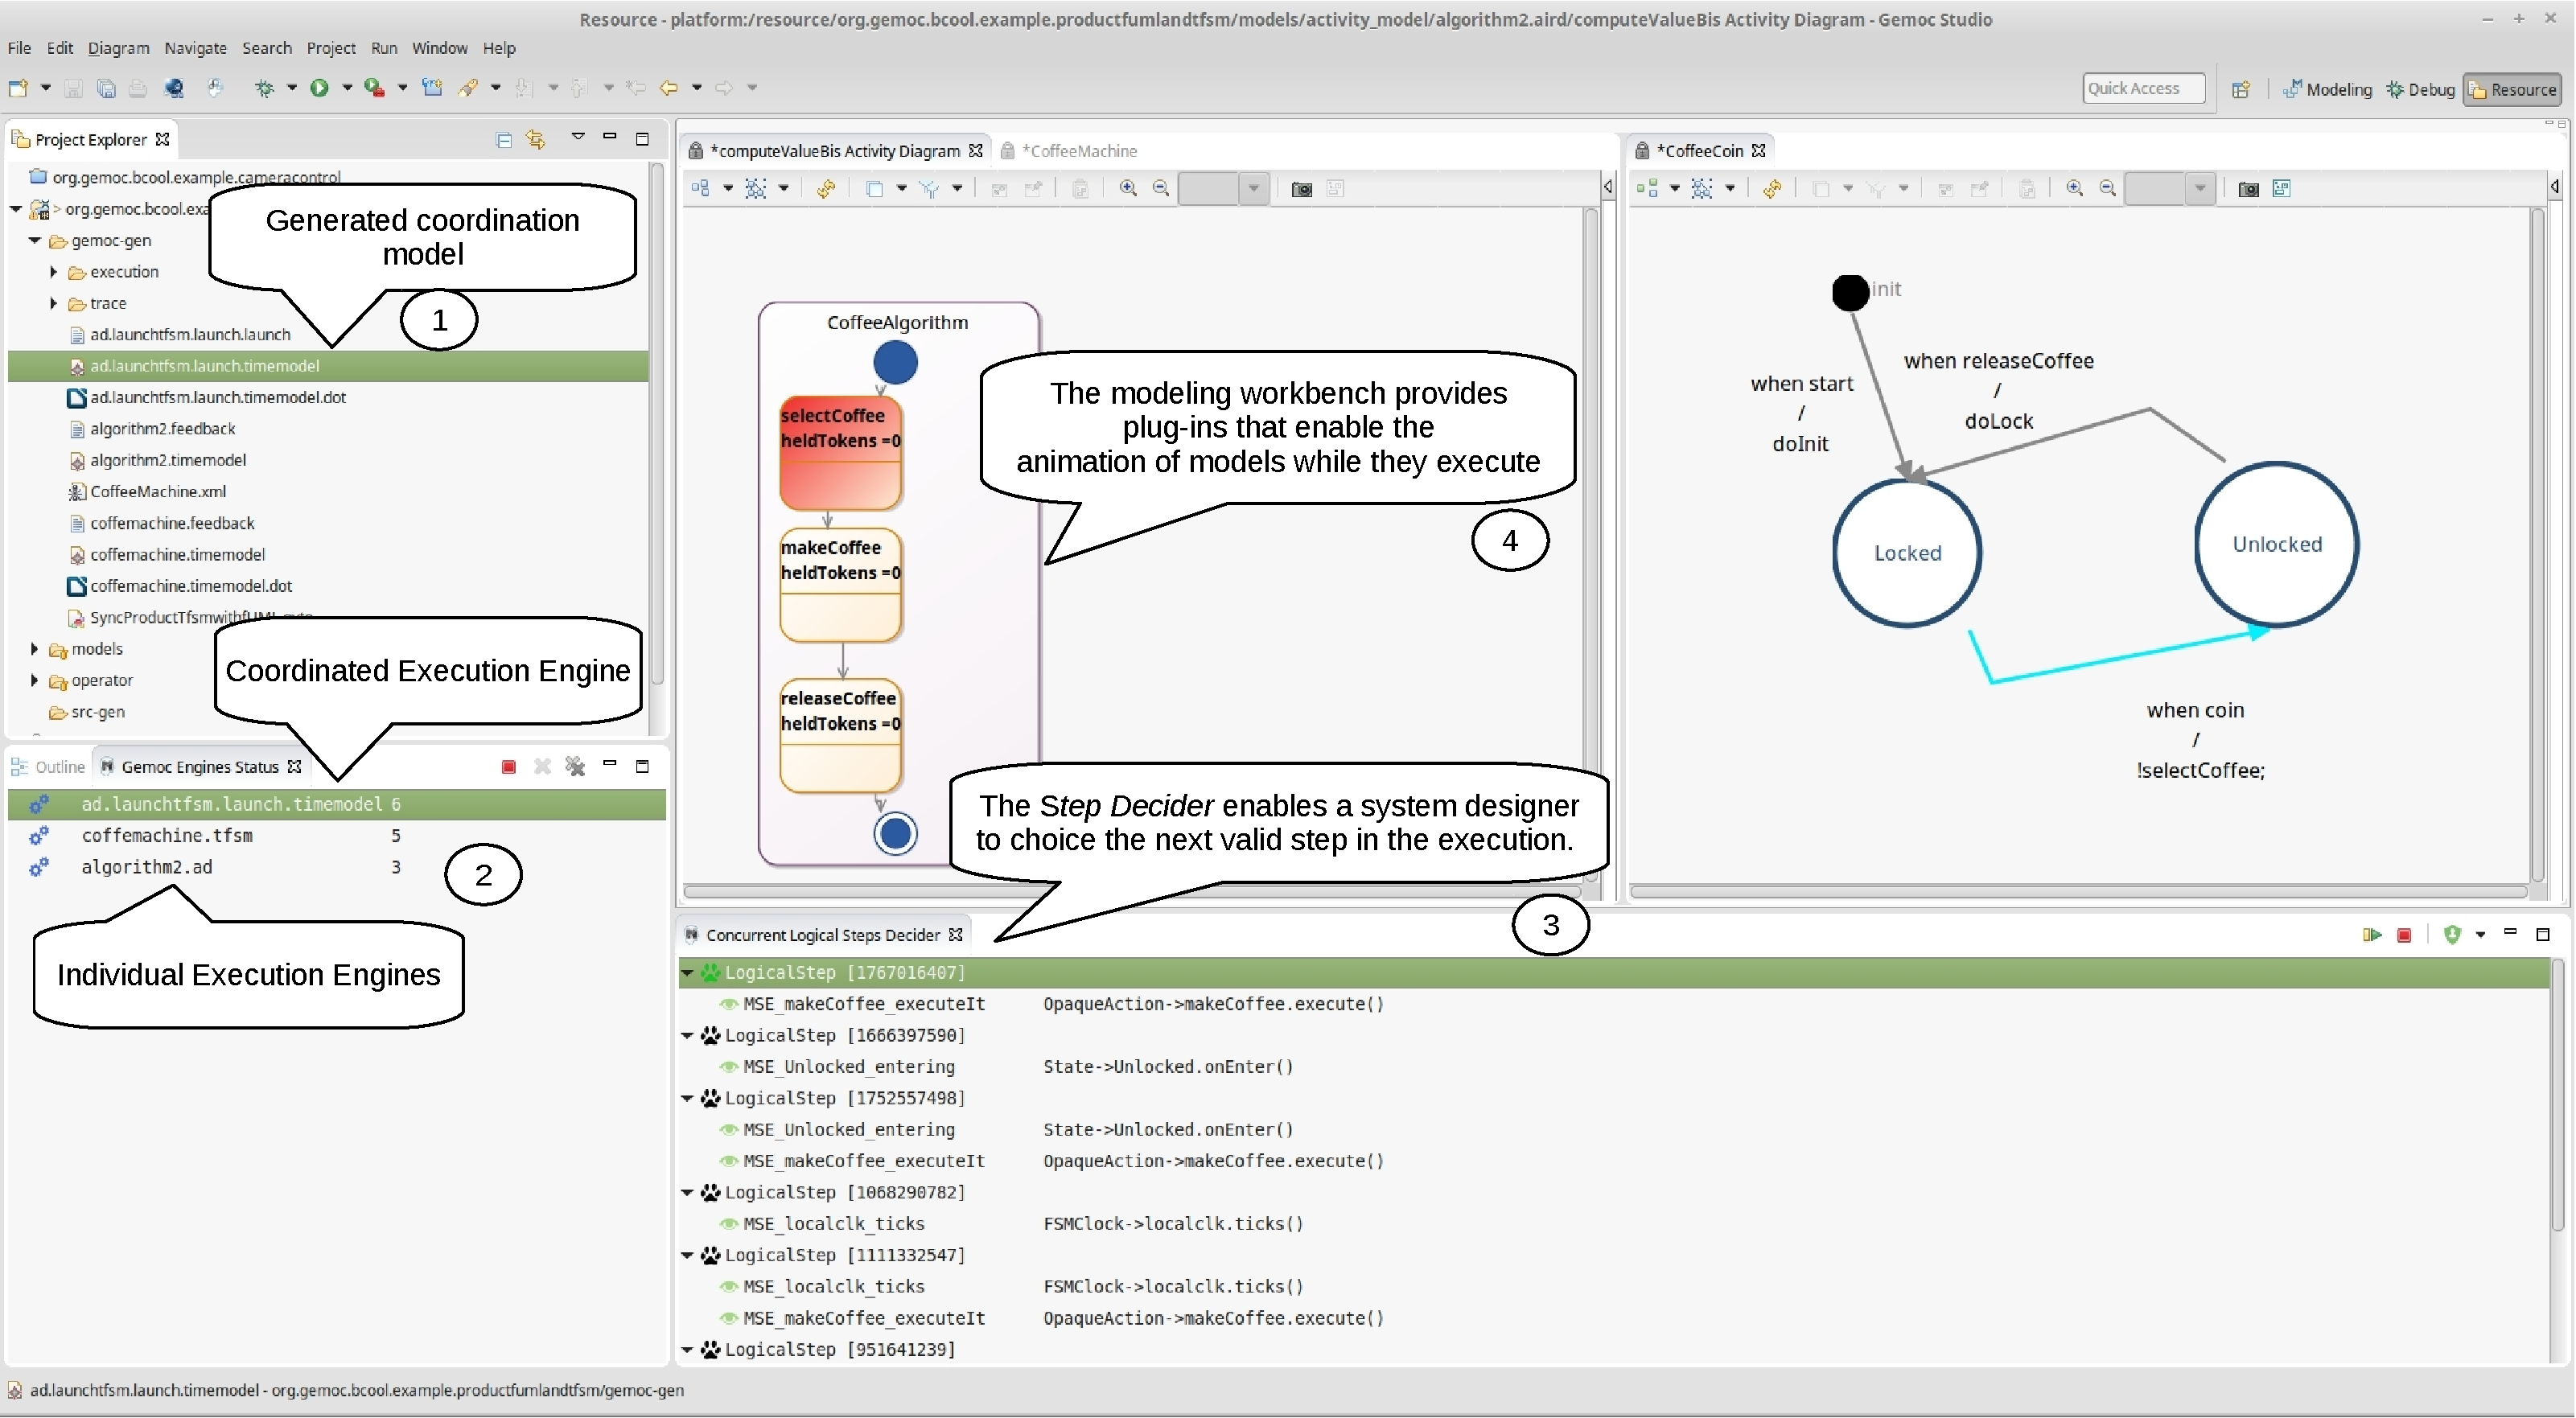
\includegraphics[width=.8\textwidth]{bcool/figs/runningworkbench}
		\label{fig:runningworkbench}
	}
	\caption{Coordinated Execution of models by using the Gemoc Coordinated Execution Engine}
	\label{fig:subfigureExample1}
\end{figure}

The project \bcool is hosted on Github\footnote{\url{http://github.com}} as part of the GEMOC project\footnote{\url{http://github.com/gemoc/coordination}}, thus making the source code publicly available. \bcool is currently integrated into the GEMOC studio\footnote{The reader can download studio the from \url{http://gemoc.org/studio-download/}}. To try the coffee machine example, the reader needs to download the studio and then to follow the tutorial from the companion website\footnote{\url{http://timesquare.inria.fr/BCOoL}}. In addition, the website contains more examples with full descriptions. %TODO:For example, it contains a video that presents the whole flow of the coffee machine example.

In this section, we have presented the implementation of \bcool into the GEMOC studio. The workbench eases the tasks of language integrators and system designers to coordinate models. Integrators can develop operators between languages that a system designer can use to coordinate, execute and validate their models. In the next section, we compare our approach with coordination languages and coordination frameworks.  

\begin{figure}[]
	\begin{center}
		\includegraphics[width=1\textwidth]{bcool/figs/statespace}
		\caption{State space representation of the coordinated model of the coffee machine, encoding the set of valid schedules. The transitions in red contain the events forced to happen simultaneously by the coordination.}
		\label{fig:statespace}
	\end{center}
\end{figure}

%\bcool is developed as set of plugins for Eclipse Modeling Framework (EMF)\footnote{http://www.eclipse.org}. Its abstract syntax has been developed using Ecore (\ie the meta-language associated with EMF) and the textual concrete  syntax has been developed in Xtext, thus providing advanced editing facilities (see Figure~\ref{fig:bcooltechnos}). A \bcool specification is defined between languages by relying on its language behavioral interface made of \dse. To get the \dse, the \ecl specification of each language must be imported (Figure~\ref{fig:bcooltechnos}: point 1). From a \bcool specification, the generation of the coordination between models has been automated by relying on two technologies: Acceleo\footnote{http://www.eclipse.org/acceleo/} and QVTo\footnote{https://projects.eclipse.org/projects/modeling.mmt.qvt-oml}. The acceleo transformation translates the \bcool specification into a QVTo transformation (Figure~\ref{fig:bcooltechnos}: point 2). The transformation can be applied between models to generate the coordination specification in \ccsl (Figure~\ref{fig:bcooltechnos}: point 3).    
	

	
%These technologies has been integrated into the GEMOC Studio, an Eclipse package atop EMF, which includes both a \emph{language workbench} to design and implement tool-supported xDSMLs, and a \emph{modeling workbench} where the xDSMLs are automatically deployed to allow system designers to edit, execute, simulate, and animate their models. In this context, \bcool takes advantages of this collaborative environment by adding coordination facilities. 

%\begin{figure}[h]
%	\begin{center}
%		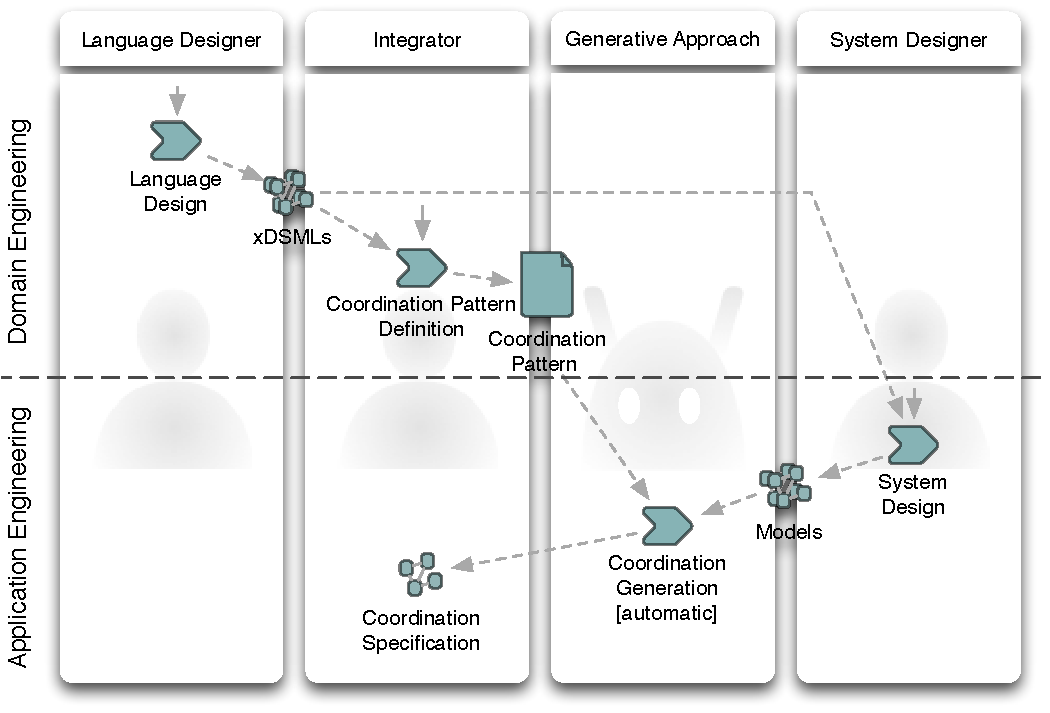
\includegraphics[width=.6\textwidth]{bcool/figs/process}
%		\caption{The Proposed Workflow}
%		\label{fig:proposedworkflow}
%	\end{center}
%\end{figure}

%Based on the GEMOC studio, Figure~\ref{fig:proposedworkflow} illustrates the proposed workflow. Such a workflow relies mainly in two stakeholders: an integrator that uses the language workbench and an system designer that uses the model workbench. 

%In the language workbench, an integrator develop operators by relying on the deployed languages. The \bcool specification can import the language behavioral interface that are automatically deployed into the workbench. To build its own libraries, the workbench provides \moccml thus helping the integrator to specify EventRelations and EventExpression. 

%Operators are automatically deployed into the modeling workbench and can be used by a system designer to generate the coordination. This task is automated by relying on a set of plugins\footnote{\todo{I have to talk about how the operators are applied by the plugin, this is not evident!}}. The workbench provides several tools to perform verification activities \eg execution and animation, space-state exploration, etc.  

%To summarize, a \bcool developer (\ie integrator) develops a set of operators by relying on the language behavioral interface (\ecl) and libraries (\moccml). Then, a \bcool user (\ie system designer) applies these operator on his models to: 
%		\begin{itemize}
%			\item Generate a coordination specification.
%			\item Perform execution and verification activities.
%		\end{itemize}

%We implement the running example in the GEMOC studio. We rely on the languages TFSM and Activity that are integrated into the study. Then, we use \bcool to specify the operator in Listing~\ref{lst:bcoolrunningexample} (Figure~\ref{fig:screenbcool}: point 1). In the model workbench, we build the models of the coffee machine: a TFSM named \emph{CoffeeCoin} and an Activity named \emph{CoffeeAlgorithm} (Figure~\ref{fig:screenbcool}: point 2). Then, we use the workbench to execute, verify and animate the coordinated models. In particular, Figure shows the animation proposed by Sirius.   

%\begin{figure}[h]
%	\begin{center}
%		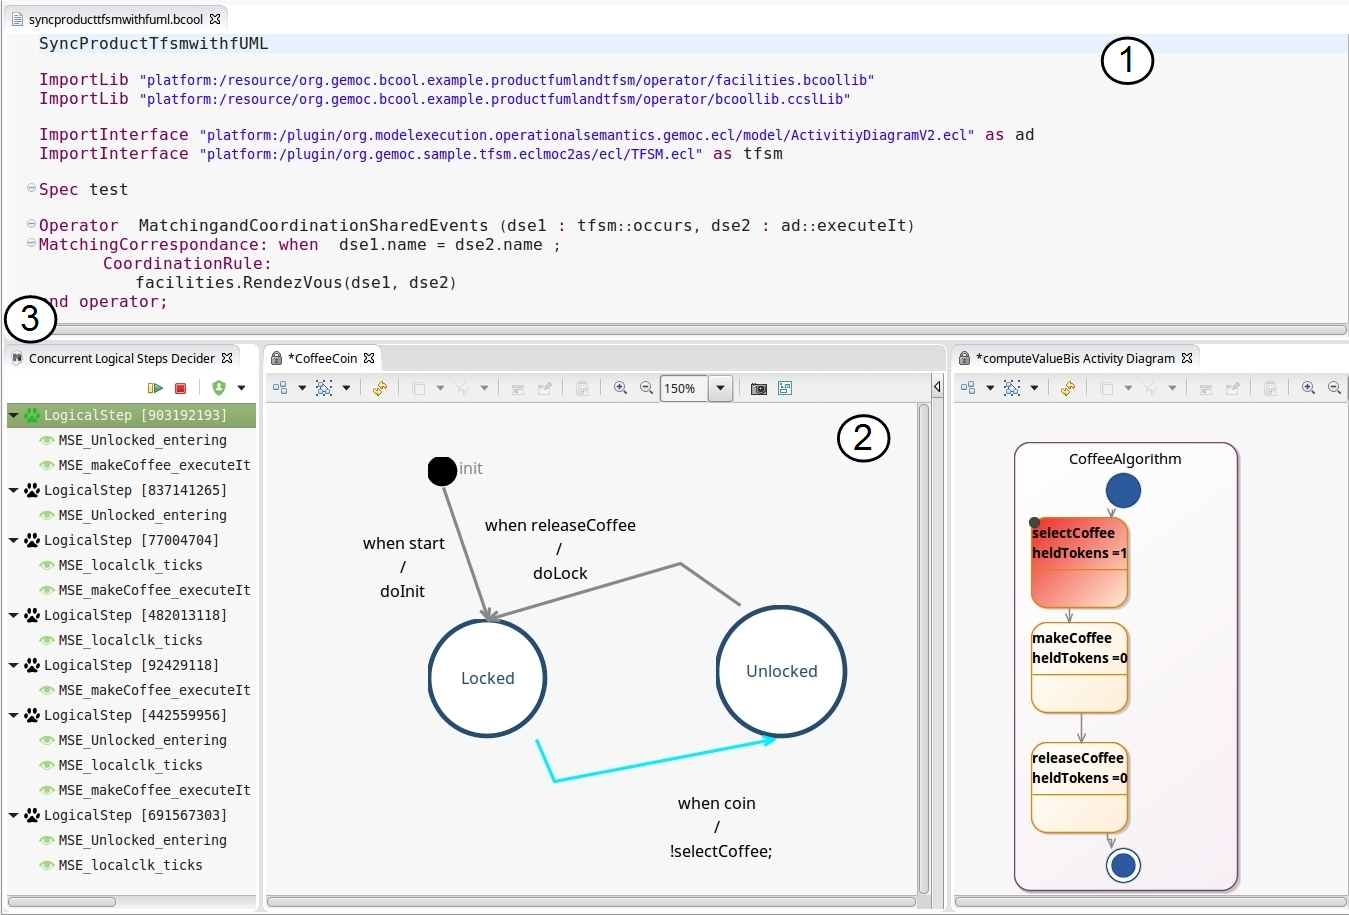
\includegraphics[width=.6\textwidth]{bcool/figs/bcoolscreen.png}
%		\caption{Screenshot}
%		\label{fig:screenbcool}
%	\end{center}
%\end{figure}

%A video presenting the whole flow can be found on the companion website~\footnote{http://timesquare.inria.fr/BCOoL}, which also contains more examples with full descriptions. These examples are hosted in Github~\footnote{http://github.com} at BCOoLExamples~\footnote{http://matiasvara.github.io/BCOoLExamples/}. The \bcool code is hosted in the open source project Gemoc~\footnote{http://github.com/gemoc/} thus making the project fully available.

%\subsection{Flow by using the plugins}
%\subsection{Flow by using ANT}
%	\begin{itemize}
%		\item Ant\footnote{http://www.eclipse.org/eclipse/ant/}
%		\item Operational QVT Ant tasks let you launch QVTO transformations from the Ant script.
%		\item The flow can be implemented by using Ant.
%		\item This enables to define explicitly how a \bcool specification is invoked. 
%		\item However, the specification of a ANT script must be partially defined by the user. For instances, several parameters must be defined by the user, \eg model paths, generated timemodel. 
		  
%	\end{itemize}


 % \begin{figure}[h]
  %	\begin{center}
  %		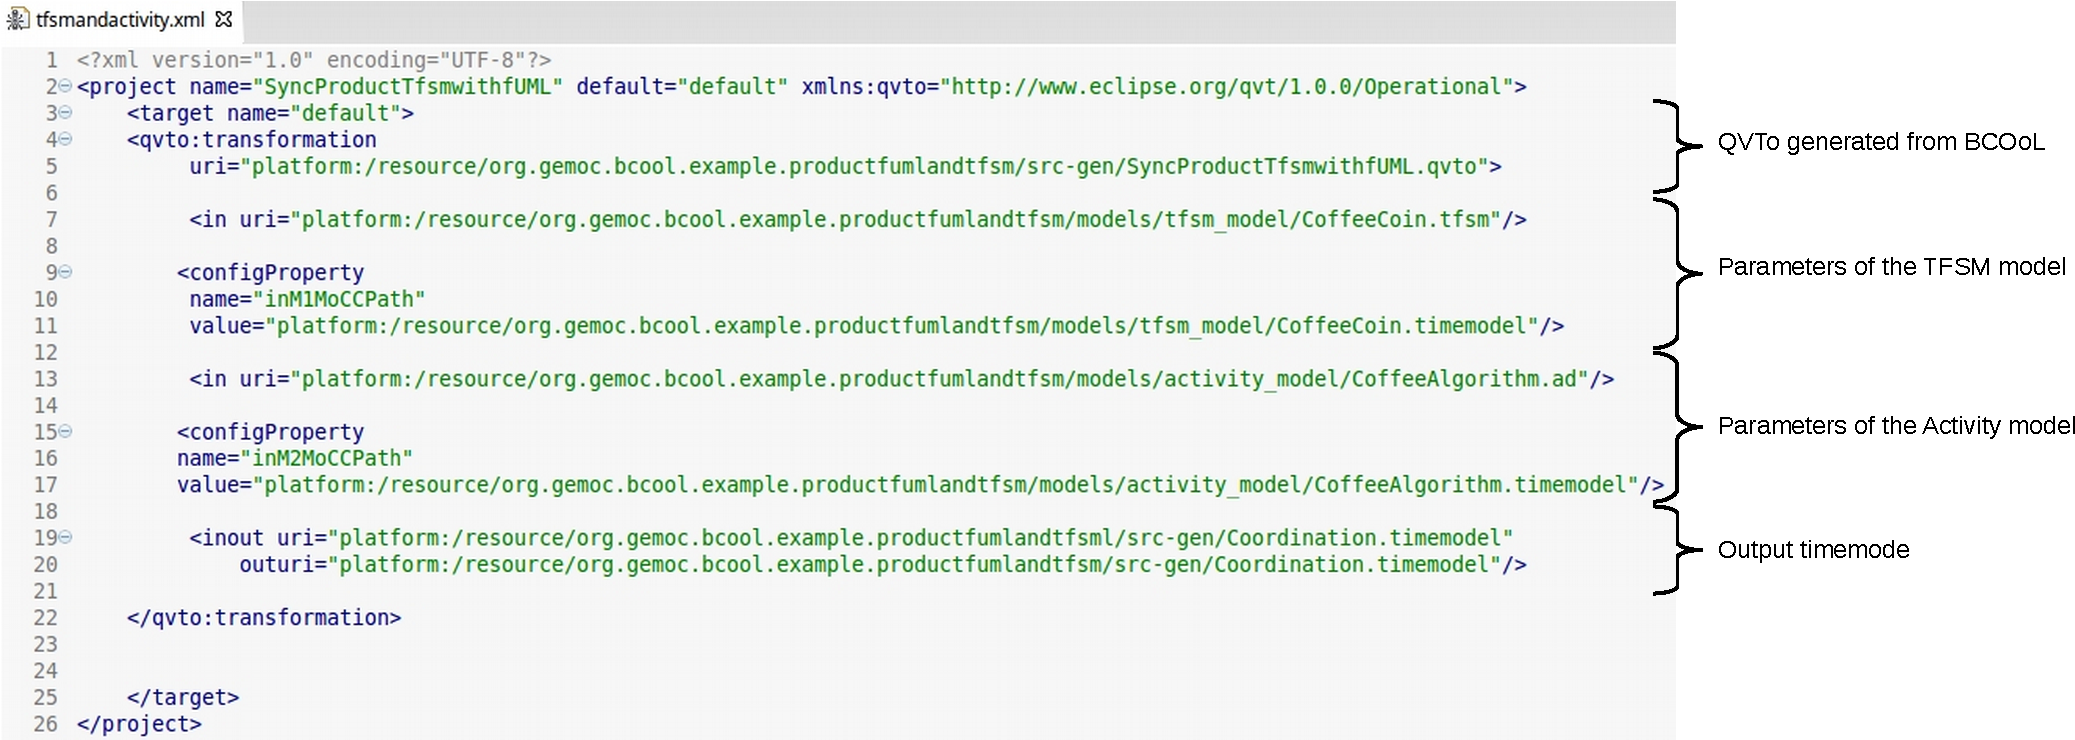
\includegraphics[width=1\textwidth]{bcool/figs/antbcool.pdf}
  %		\caption{ANT script to build the coordination specification for the coffee machine}
  %		\label{fig:screenantbcool}
 % 	\end{center}
 % \end{figure}